\documentclass[11pt]{article}
\usepackage{amsmath,textcomp,amssymb,geometry,graphicx,enumerate,tikz}

\def\Name{Vijay Hans}  % Your name
\def\SID{3041285081}  % Your student ID number
\def\Prelab{8} % Number of Prelab
\def\Session{Spring 2026}
\def\Cls{PHYS 5BL}
\title{\Cls--Spring 2026 --- Prelab \Prelab \ Response}
\author{\Name, SID \SID}
\markboth{\Cls -- \Session\  Prelab \Prelab \ \Name}{\Cls -- \Session\ Prelab \Prelab\ \Name}
\pagestyle{myheadings}
\date{\today}

\newenvironment{qparts}{\begin{enumerate}[{(}a{)}]}{\end{enumerate}}
\def\endproofmark{$\Box$}
\newenvironment{proof}{\par{\bf Proof}:}{\endproofmark\smallskip}

\textheight=9in
\textwidth=6.5in
\topmargin=-.75in
\oddsidemargin=0.25in
\evensidemargin=0.25in
\setlength{\parindent}{0pt}
\begin{document}
\maketitle
\begin{enumerate}
    \item 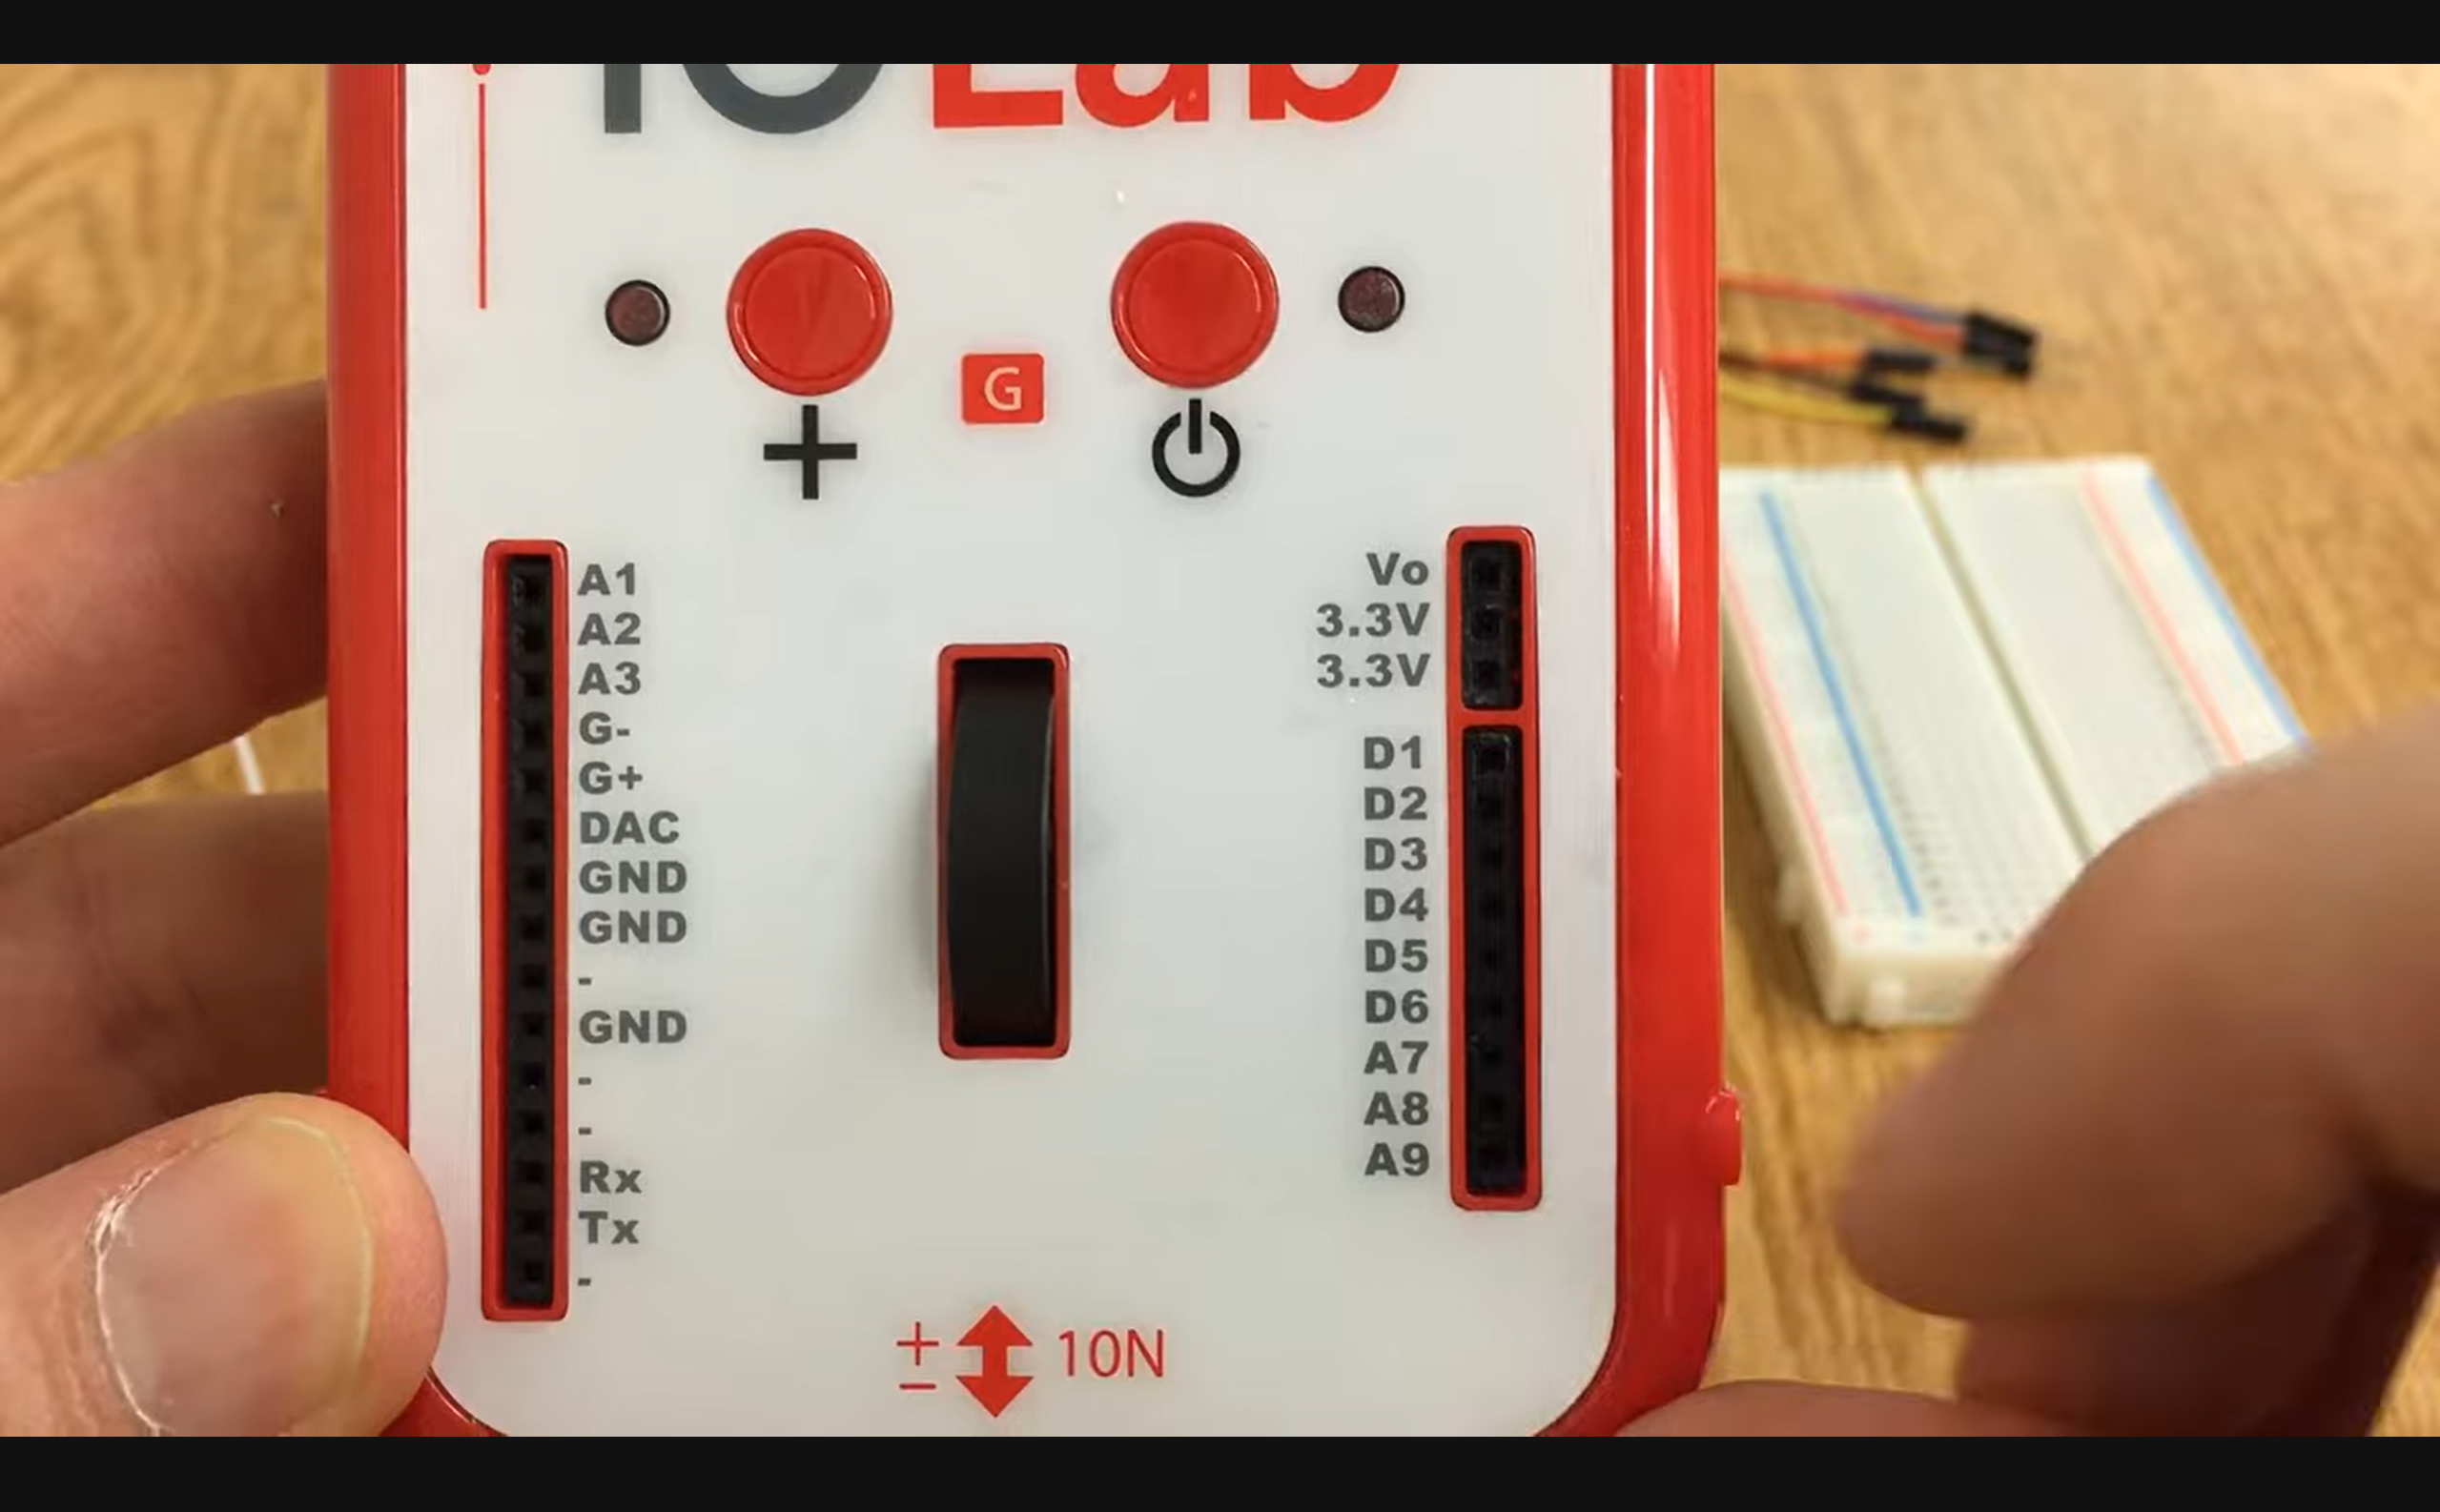
\includegraphics[scale=0.2]{prelab video graphic.png}
    \item We have a 5-band resistor, so we have 3 digits of precision with our resistance reading. Red-Green-Black corresponds to 250, Blue gives a multiplier of 1M, and Gold gives a tolerance of $\pm 5 \%$. Thus the resistance is $250 \pm 12.5 M\Omega$.
    \item Let the resistors have resistances $R_1, R_2$. Let the total current passing through them be $I$ and let the current passing through $R_1$ be $x$; by Kirchoff's Junction Rule, the current passing through $R_2$ is $I-x$. We seek to show that minimizing the power dissipated is equivalent to the standard prediction for resistors in parallel; namely, that such minimization will result in the potential difference being equal across the resistors. \\ The power dissipated through each resistor will be $I_iV_i$, which by Ohm's Law is equal to $I_i^2 R_i$. Thus the total power dissipated is $P(x) = x^2 R_1 + (I-x)^2R_2$. \\ Differentiating this with respect to $x$ gives $P'(x) = 2xR_1 - 2(I-x)R_2$, which we hope to set equal to 0. Solving for $x$ gives $x = \frac{IR_2}{R_1+R_2}$ and $I-x = \frac{IR_1}{R_1+R_2}$. \\ We can verify that this is a minimum via the second derivative test: $P''(x) = 2R_1 + 2R_2$ is always positive, so we must have that $x$ is a minimum of $P$. \\ The potential difference across each resistor is $I_iR_i$. For the first resistor this is $xR_1 = \frac{IR_2}{R_1 + R_2} = \frac{IR_1R_2}{R_1+R_2}$; for the second, this is $(I-x)R_2 = \frac{IR_1}{R_1+R_2}R_2 = \frac{IR_1R_2}{R_1+R_2}$. These potential differences are equal and thus correspond to our traditional prediction for currents across parallel resistors. Thus resistors in parallel have currents distributed such that they minimize the total power dissipated.
\end{enumerate}
\end{document}